% ResNet-18 / CIFAR-10 part of the presentation (second presenter: no title page, no general introduction).
% Compile: pdflatex presentation.tex (twice).  Standard packages only (beamer, amsmath, booktabs, graphicx, colortbl).
% MobileNetV2 slides were removed for now; they are in the git history (commit c675d27 and earlier).
\documentclass[aspectratio=169,10pt]{beamer}
\usetheme{default}
\usecolortheme{default}
\usepackage[utf8]{inputenc}
\usepackage[T1]{fontenc}
\usepackage{amsmath,amssymb}
\usepackage{booktabs}
\usepackage{graphicx}
\usepackage{array}
\usepackage{colortbl}
\graphicspath{{figures/}}

\definecolor{ink}{RGB}{11,11,11}
\definecolor{accent}{RGB}{42,120,214}
\definecolor{hl}{RGB}{255,236,170}
\setbeamercolor{frametitle}{fg=ink}
\setbeamercolor{structure}{fg=accent}
\setbeamercolor{block title}{fg=white,bg=accent}
\setbeamercolor{block body}{bg=accent!8}
\setbeamerfont{frametitle}{series=\bfseries,size=\large}
\setbeamertemplate{navigation symbols}{}
\setbeamertemplate{footline}{\hfill\insertframenumber\,/\,\inserttotalframenumber\hspace{2mm}\vspace{1mm}}
\setbeamertemplate{itemize items}[circle]
\newcommand{\hlrow}{\rowcolor{hl}}

\begin{document}

% ------------------------------------------------------------------ 1. baseline
\begin{frame}{Experiment 1: ResNet-18 on CIFAR-10, the FP32 baseline}
  \begin{columns}[T]
    \begin{column}{0.49\textwidth}
      \textbf{Model and data}\\[1mm]
      \small
      \begin{tabular}{@{}ll@{}}
        \toprule
        architecture & ResNet-18, CIFAR variant (3$\times$3 stem, no max-pool)\\
        Conv/Linear layers (quantized) & 21\\
        parameters & 11\,173\,962\\
        \quad quantized weights & 11\,164\,352\\
        \quad biases + BatchNorm (kept FP32) & 9\,610\\
        FP32 weight storage & 44\,657\,408 B (44.7 MB)\\
        classes & 10\\
        images: train / validation / test & 45\,000 / 5\,000 / 10\,000\\
        training & from scratch, 200 epochs\\
        \bottomrule
      \end{tabular}\\[3mm]
      \textbf{Range of the trained weights}\\[1mm]
      \begin{tabular}{@{}lr@{}}
        \toprule
        minimum / maximum & $-0.411$ / $+0.556$\\
        mean / standard deviation & $-0.0005$ / $0.0064$\\
        std per layer (conv1 $\to$ layer4) & $0.067 \to 0.0014$ (fc 0.081)\\
        weights with $|w|<2^{-7}$ & 87.2\,\%\\
        \bottomrule
      \end{tabular}
    \end{column}
    \begin{column}{0.49\textwidth}
      \textbf{Baseline accuracy} (highlighted = the reference values used everywhere later)\\[1mm]
      \small
      \begin{tabular}{@{}lrrr@{}}
        \toprule
        split & images & accuracy & cross-entropy\\
        \midrule
        \hlrow \textbf{test (official)} & 10\,000 & \textbf{95.11\,\%} & 0.1855\\
        \hlrow \textbf{validation (holdout)} & 5\,000 & \textbf{95.48\,\%} & 0.1704\\
        \bottomrule
      \end{tabular}\\[3mm]
      \textbf{SQNR after training}\\[1mm]
      \begin{tabular}{@{}lr@{}}
        \toprule
        \hlrow \textbf{FP32 trained weights (reference)} & \textbf{$+\infty$ dB}\\
        \bottomrule
      \end{tabular}\\[1mm]
      \footnotesize The trained FP32 weights are the reference, so their quantization error is 0 and SQNR is $+\infty$.
      Every SQNR on the next slides is measured against these weights.\\[3mm]
      \small
      \textbf{Reading}
      \begin{itemize}\footnotesize
        \item Weights are small, and shrink with depth: layer4 holds 75\,\% of all weights with std below 0.0064.
        \item Weakest class: cat (88.4\,\%), mostly confused with dog.
        \item Validation and test accuracy differ by 0.37 pp, within noise of a 5\,000-image set (std.\ error about 0.3 pp).
      \end{itemize}
    \end{column}
  \end{columns}
\end{frame}

% ------------------------------------------------------------------ 2. datatype table
\begin{frame}{Clean quantization: every layer stored in one format}
  \centering
  \small
  Weights-only quantization, FP32 compute on the decoded weights; validation set of 5\,000 images.\\[3mm]
  \begin{tabular}{@{}lrrrr@{}}
    \toprule
    datatype & bit/weight & validation accuracy & drop from FP32 (pp) & global SQNR (dB)\\
    \midrule
    \hlrow \textbf{FP32 (baseline)} & 32 & \textbf{95.48\,\%} & -- & $+\infty$\\
    E4M11-SN & 16 & 95.48\,\% & 0.00 & 69.27\\
    FP16 (IEEE binary16) & 16 & 95.48\,\% & 0.00 & 73.67\\
    FP8 E4M3FN & 8 & 95.30\,\% & 0.18 & 21.20\\
    INT8 (per-tensor) & 8 & 95.36\,\% & 0.12 & 32.58\\
    INT4 (per-tensor) & 4 & 94.30\,\% & 1.18 & 7.85\\
    \bottomrule
  \end{tabular}\\[4mm]
  \begin{itemize}\small
    \item SQNR $=10\log_{10}\dfrac{\sum_i w_i^2}{\sum_i (w_i-\hat w_i)^2}$ over all 21 layers pooled; $\hat w_i$ = weight decoded from the stored format.
    \item E4M11-SN and FP16 reproduce FP32 exactly; INT8 and FP8 lose at most 0.18 pp; only INT4 loses clearly (1.18 pp).
    \item \textbf{SQNR does not rank accuracy}: FP8 (21.2 dB) and INT8 (32.6 dB) are within 0.2 pp of each other; INT4 (7.85 dB) loses 1.18 pp.
  \end{itemize}
\end{frame}

% ------------------------------------------------------------------ 3. optimization
\begin{frame}{Optimization function: which format for which layer?}
  Choose one datatype $d$ for every layer $l$ (binary $x_{l,d}$):
  \[
    \min_{x}\ \sum_{l}\sum_{d} x_{l,d}\Big(\widetilde{Q}(l,d)+\lambda\,\widetilde{R}(l,d)\Big)
    \quad\text{s.t.}\quad \sum_{d} x_{l,d}=1\ \ \forall l,\qquad \sum_{l,d} x_{l,d}\,S(l,d)\le B\cdot\tfrac{N}{8}
  \]
  \vspace{-3mm}
  {\footnotesize $\widetilde{\cdot}$ = min--max normalised, $\lambda=1$, $N$ = number of quantized weights, budget $B=8$ bit/weight. Solved exactly as an integer linear programme (HiGHS); every solution is then assembled and measured end to end.}
  \vspace{1mm}
  \begin{columns}[T]
    \begin{column}{0.33\textwidth}
      \begin{block}{$Q$: quantization penalty}
        \small
        $Q(l,d)=\sum_{i\in l}F_i\,(w_i-\hat w_i)^2$\\[1mm]
        Rounding error of layer $l$ in format $d$, weighted by the \textbf{Fisher information} $F_i$ (how sharply the loss curves in the direction of weight $i$).
        Large for coarse formats in sensitive layers.
      \end{block}
    \end{column}
    \begin{column}{0.33\textwidth}
      \begin{block}{$R$: fault risk}
        \small
        $R(l,d)\approx$ accuracy drop when random bits of layer $l$ stored in format $d$ flip (8 flips)\\[1mm]
        Measured by fault injection into the stored bytes. Large for float formats with exponent bits (FP16), tiny for INT.
      \end{block}
    \end{column}
    \begin{column}{0.33\textwidth}
      \begin{block}{$S$: storage}
        \small
        $S(l,d)$ = real stored bytes of layer $l$ in format $d$ (payload + scales)\\[1mm]
        E4M11, FP16: 16 bit; FP8, INT8: 8 bit; INT4: 4 bit per weight.
        The budget keeps the whole model $\le 8$ bit/weight on average.
      \end{block}
    \end{column}
  \end{columns}
  \vspace{1mm}
  {\footnotesize $Q$ and $R$ pull in opposite directions: $Q$ favours fine formats, $R$ favours formats whose bits are harmless to flip, and $S$ limits the size.}
\end{frame}

% ------------------------------------------------------------------ 4. heatmaps
\begin{frame}{Where do bit flips hurt? Accuracy lost per layer and format}
  \centering
  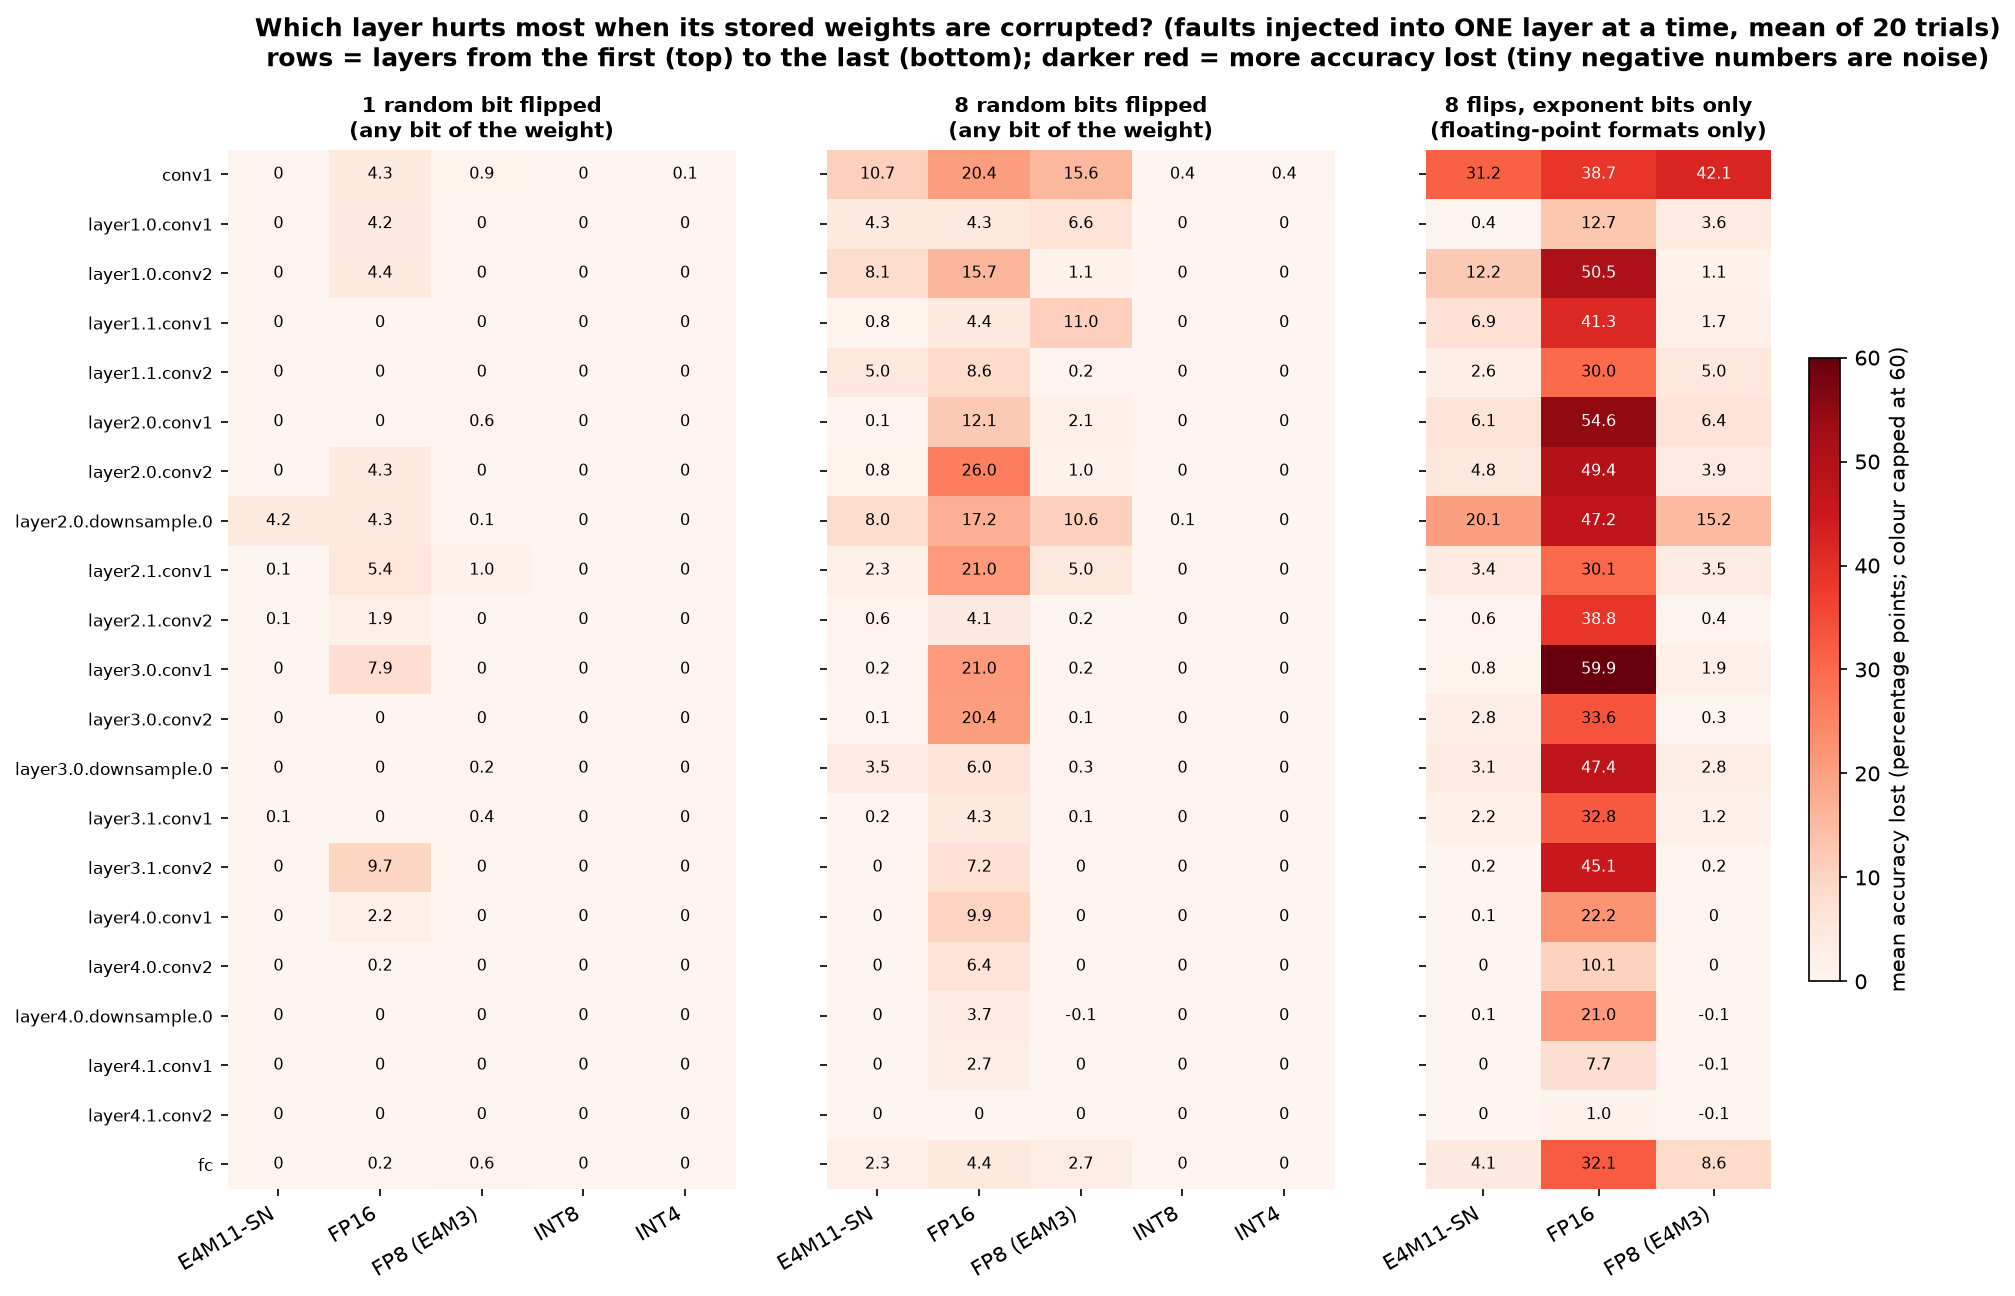
\includegraphics[width=0.78\textwidth,height=0.77\textheight,keepaspectratio]{rn_layer_heatmaps.png}\\[-1mm]
  {\scriptsize Faults injected into one layer at a time, mean of 20 trials. INT8 and INT4 weights are almost unaffected; FP16 is the most fragile, and exponent-bit flips are the worst.
  The first layers (conv1) are the most exposed. This is the measurement behind $R$.}
\end{frame}

% ------------------------------------------------------------------ 5. feature maps
\begin{frame}{What the layers see: feature maps with weights in different formats}
  \centering
  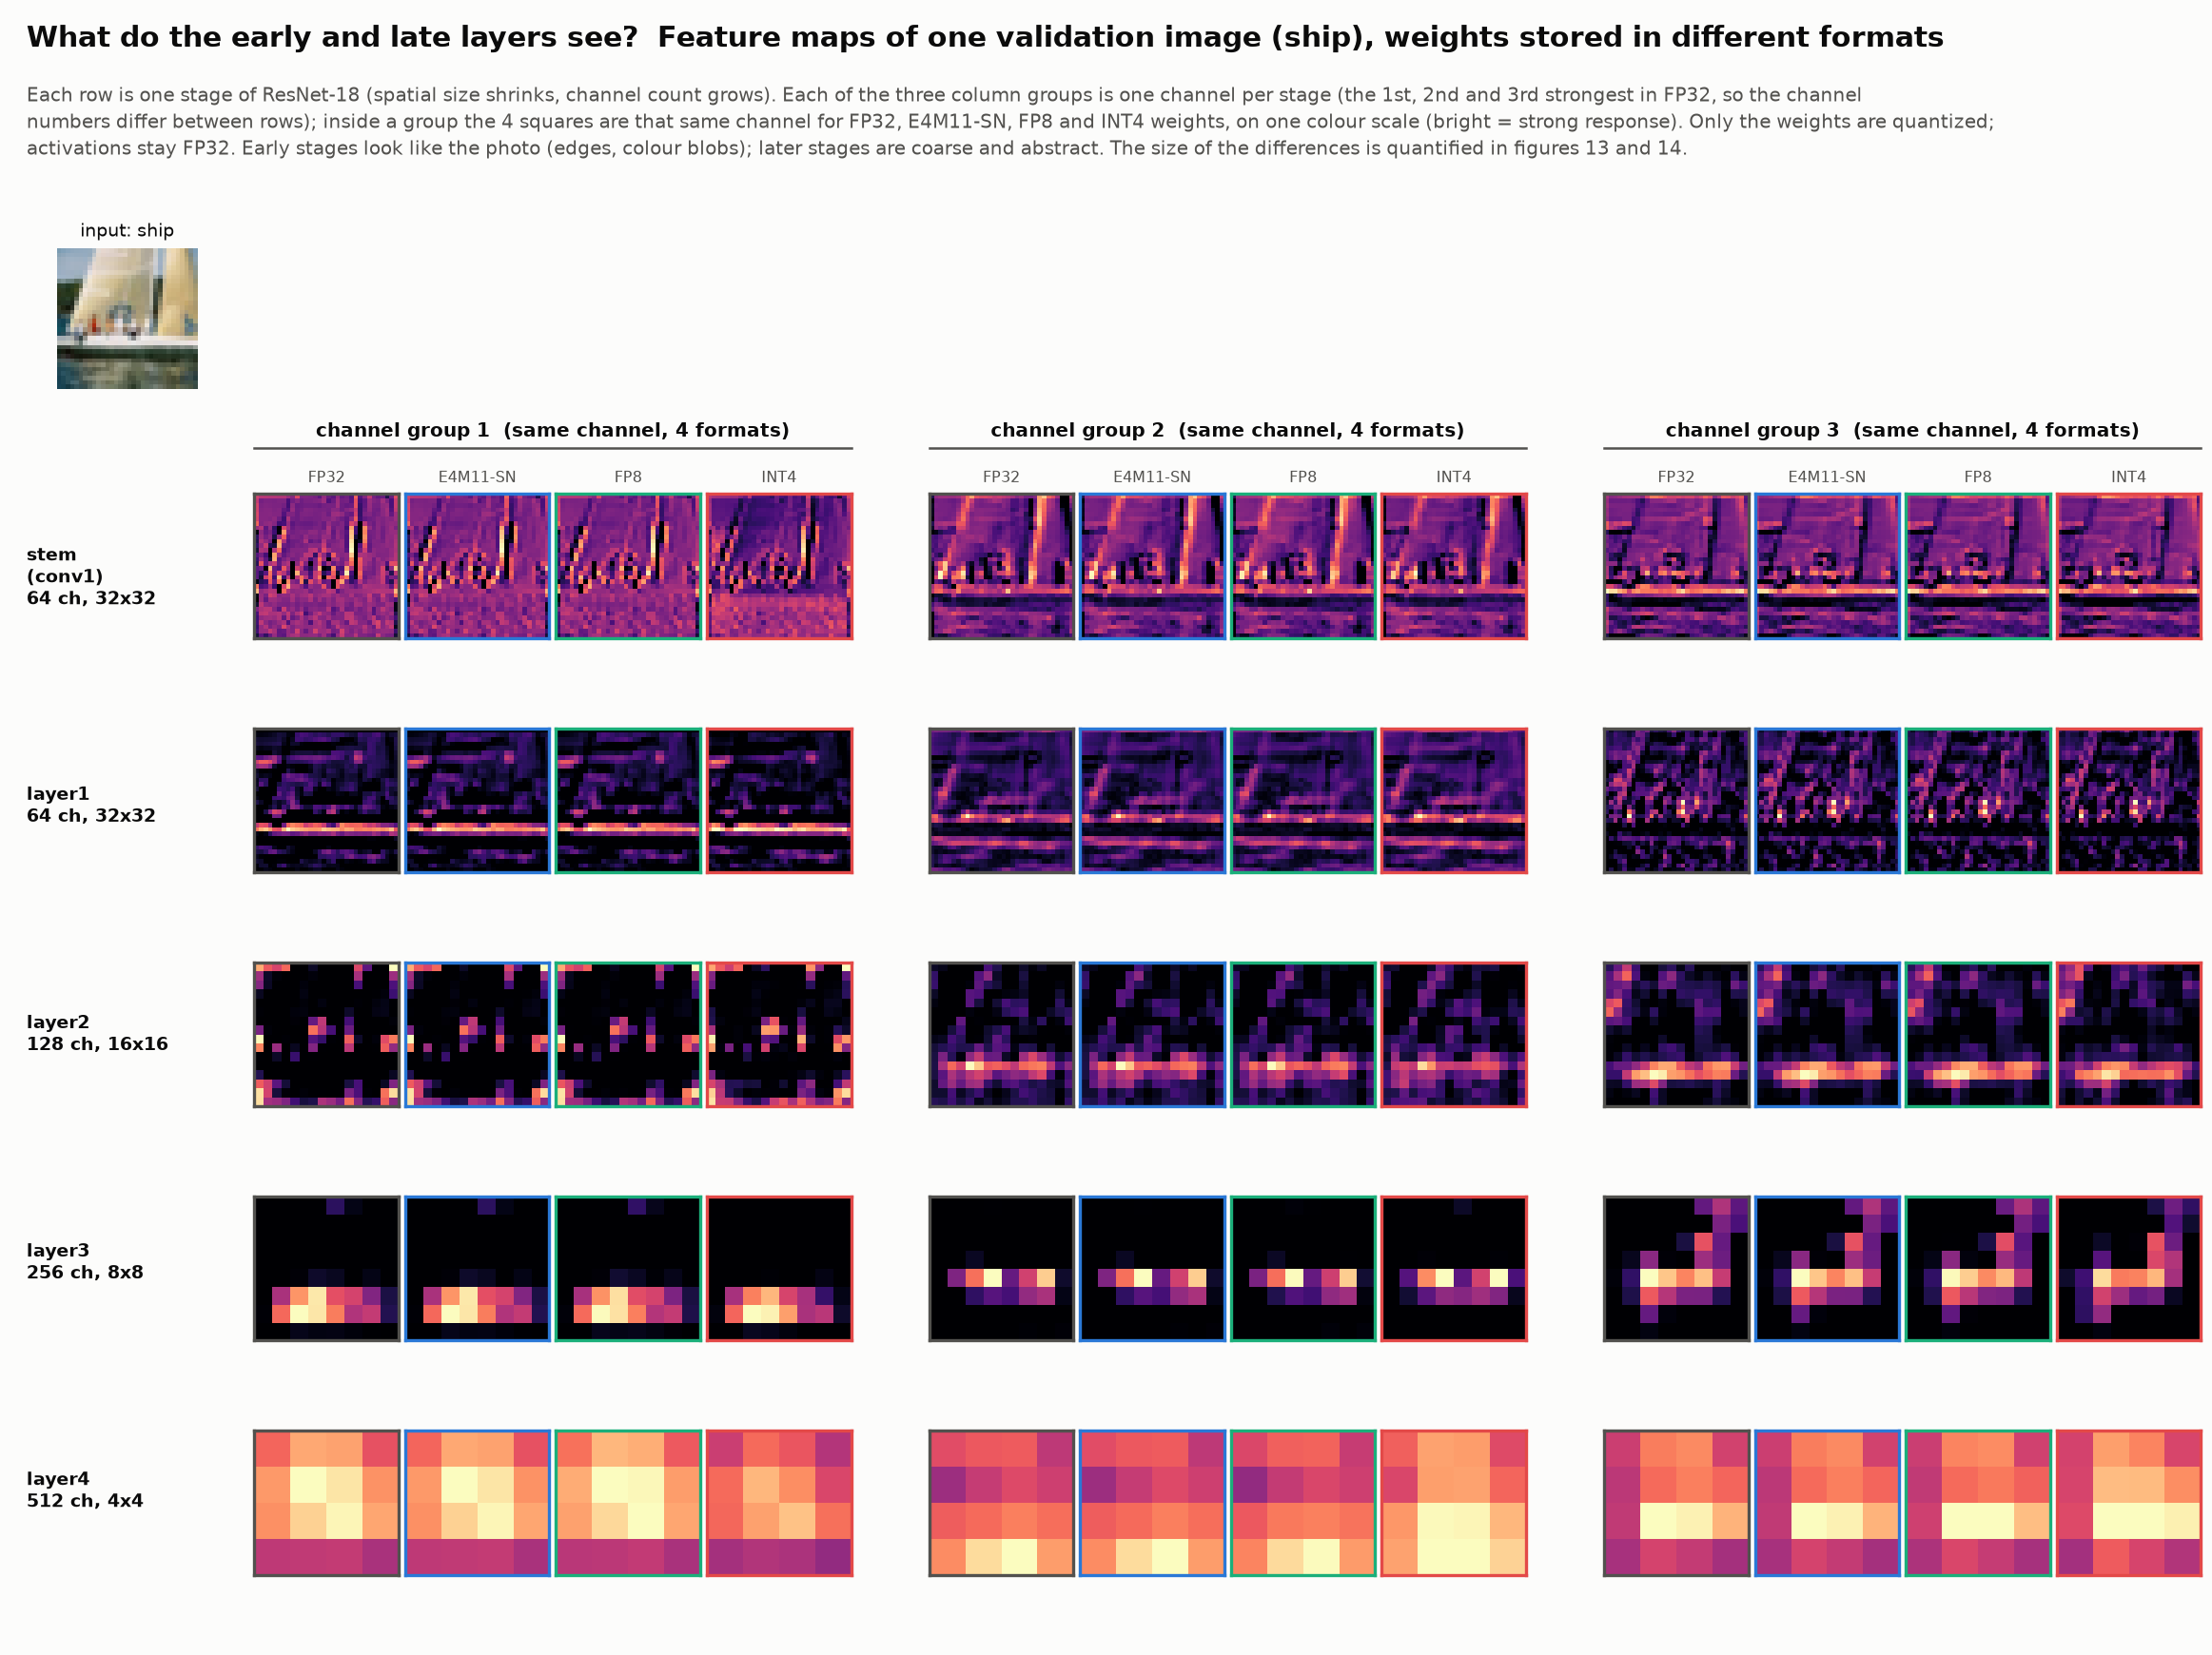
\includegraphics[width=0.66\textwidth,height=0.78\textheight,keepaspectratio]{rn_feature_maps.png}\\[-1mm]
  {\scriptsize One validation image (ship); per stage, three channels shown for FP32, E4M11-SN, FP8 and INT4 weights. Only weights are quantized.
  E4M11-SN and FP8 are nearly identical to FP32; INT4 deviates more, visibly in the early stages. Early stages look like the photo, later stages are coarse and abstract.}
\end{frame}

% ------------------------------------------------------------------ 6. Fisher
\begin{frame}{Fisher sensitivity of each layer: ResNet-18}
  \centering
  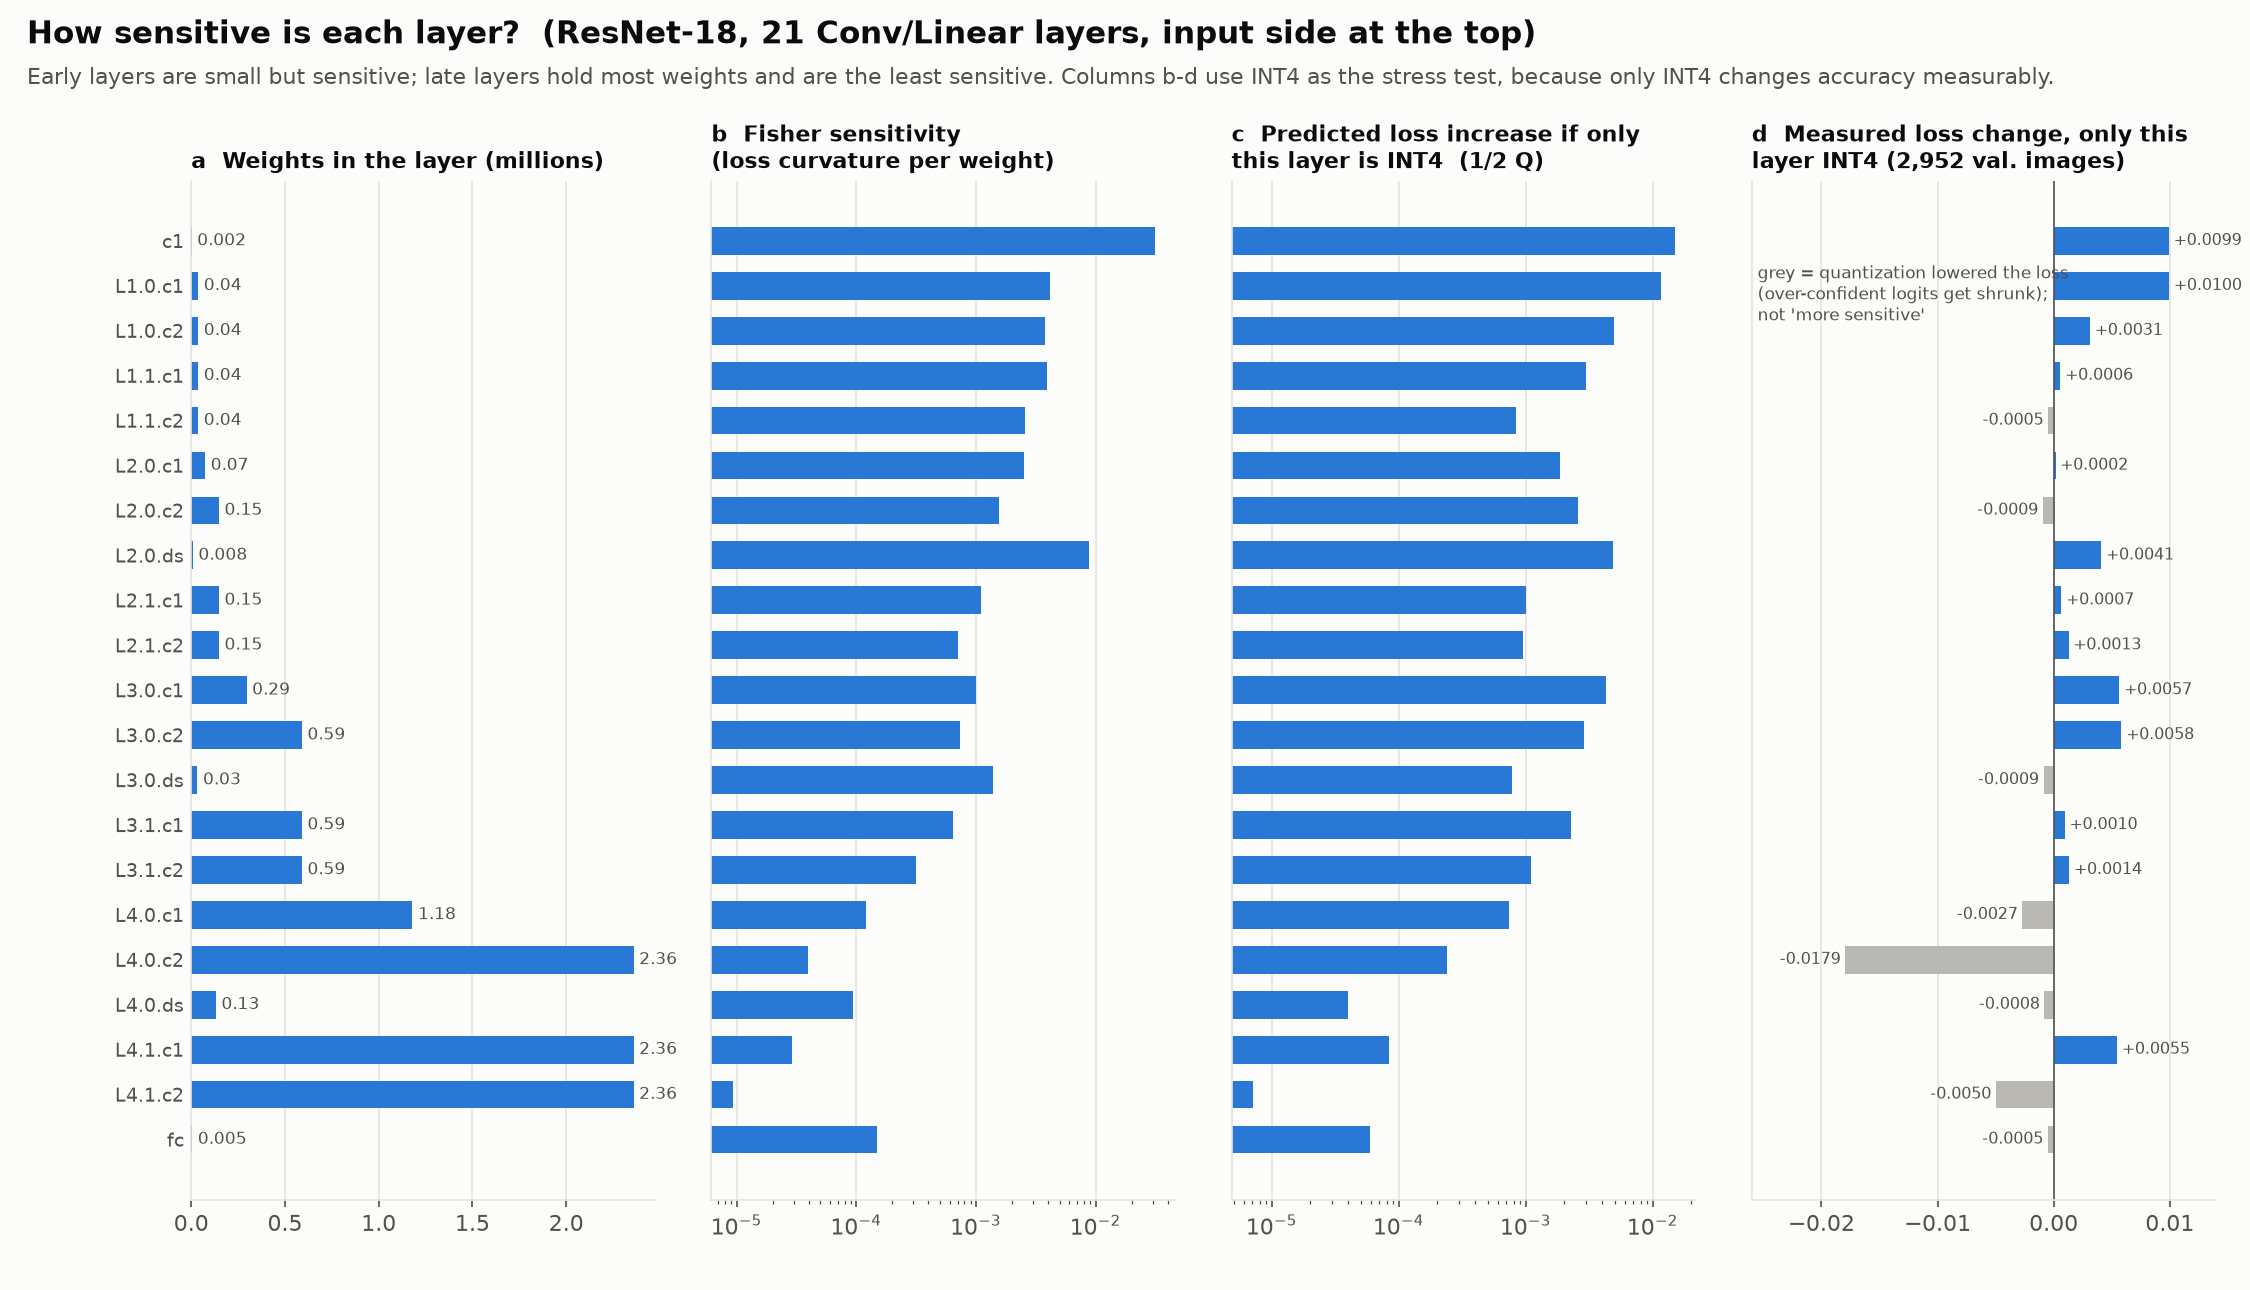
\includegraphics[width=0.97\textwidth,height=0.78\textheight,keepaspectratio]{rn_sensitivity_profile.png}\\[-1mm]
  {\scriptsize b = Fisher per weight (log), c = predicted loss increase $\tfrac12 Q$ if only this layer is INT4, d = measured. Early layers are small but sensitive; late layers hold most weights and are least sensitive.}
\end{frame}

% ------------------------------------------------------------------ 7. A051 figure
\begin{frame}{Selected assignment A051: which format does each layer get?}
  \centering
  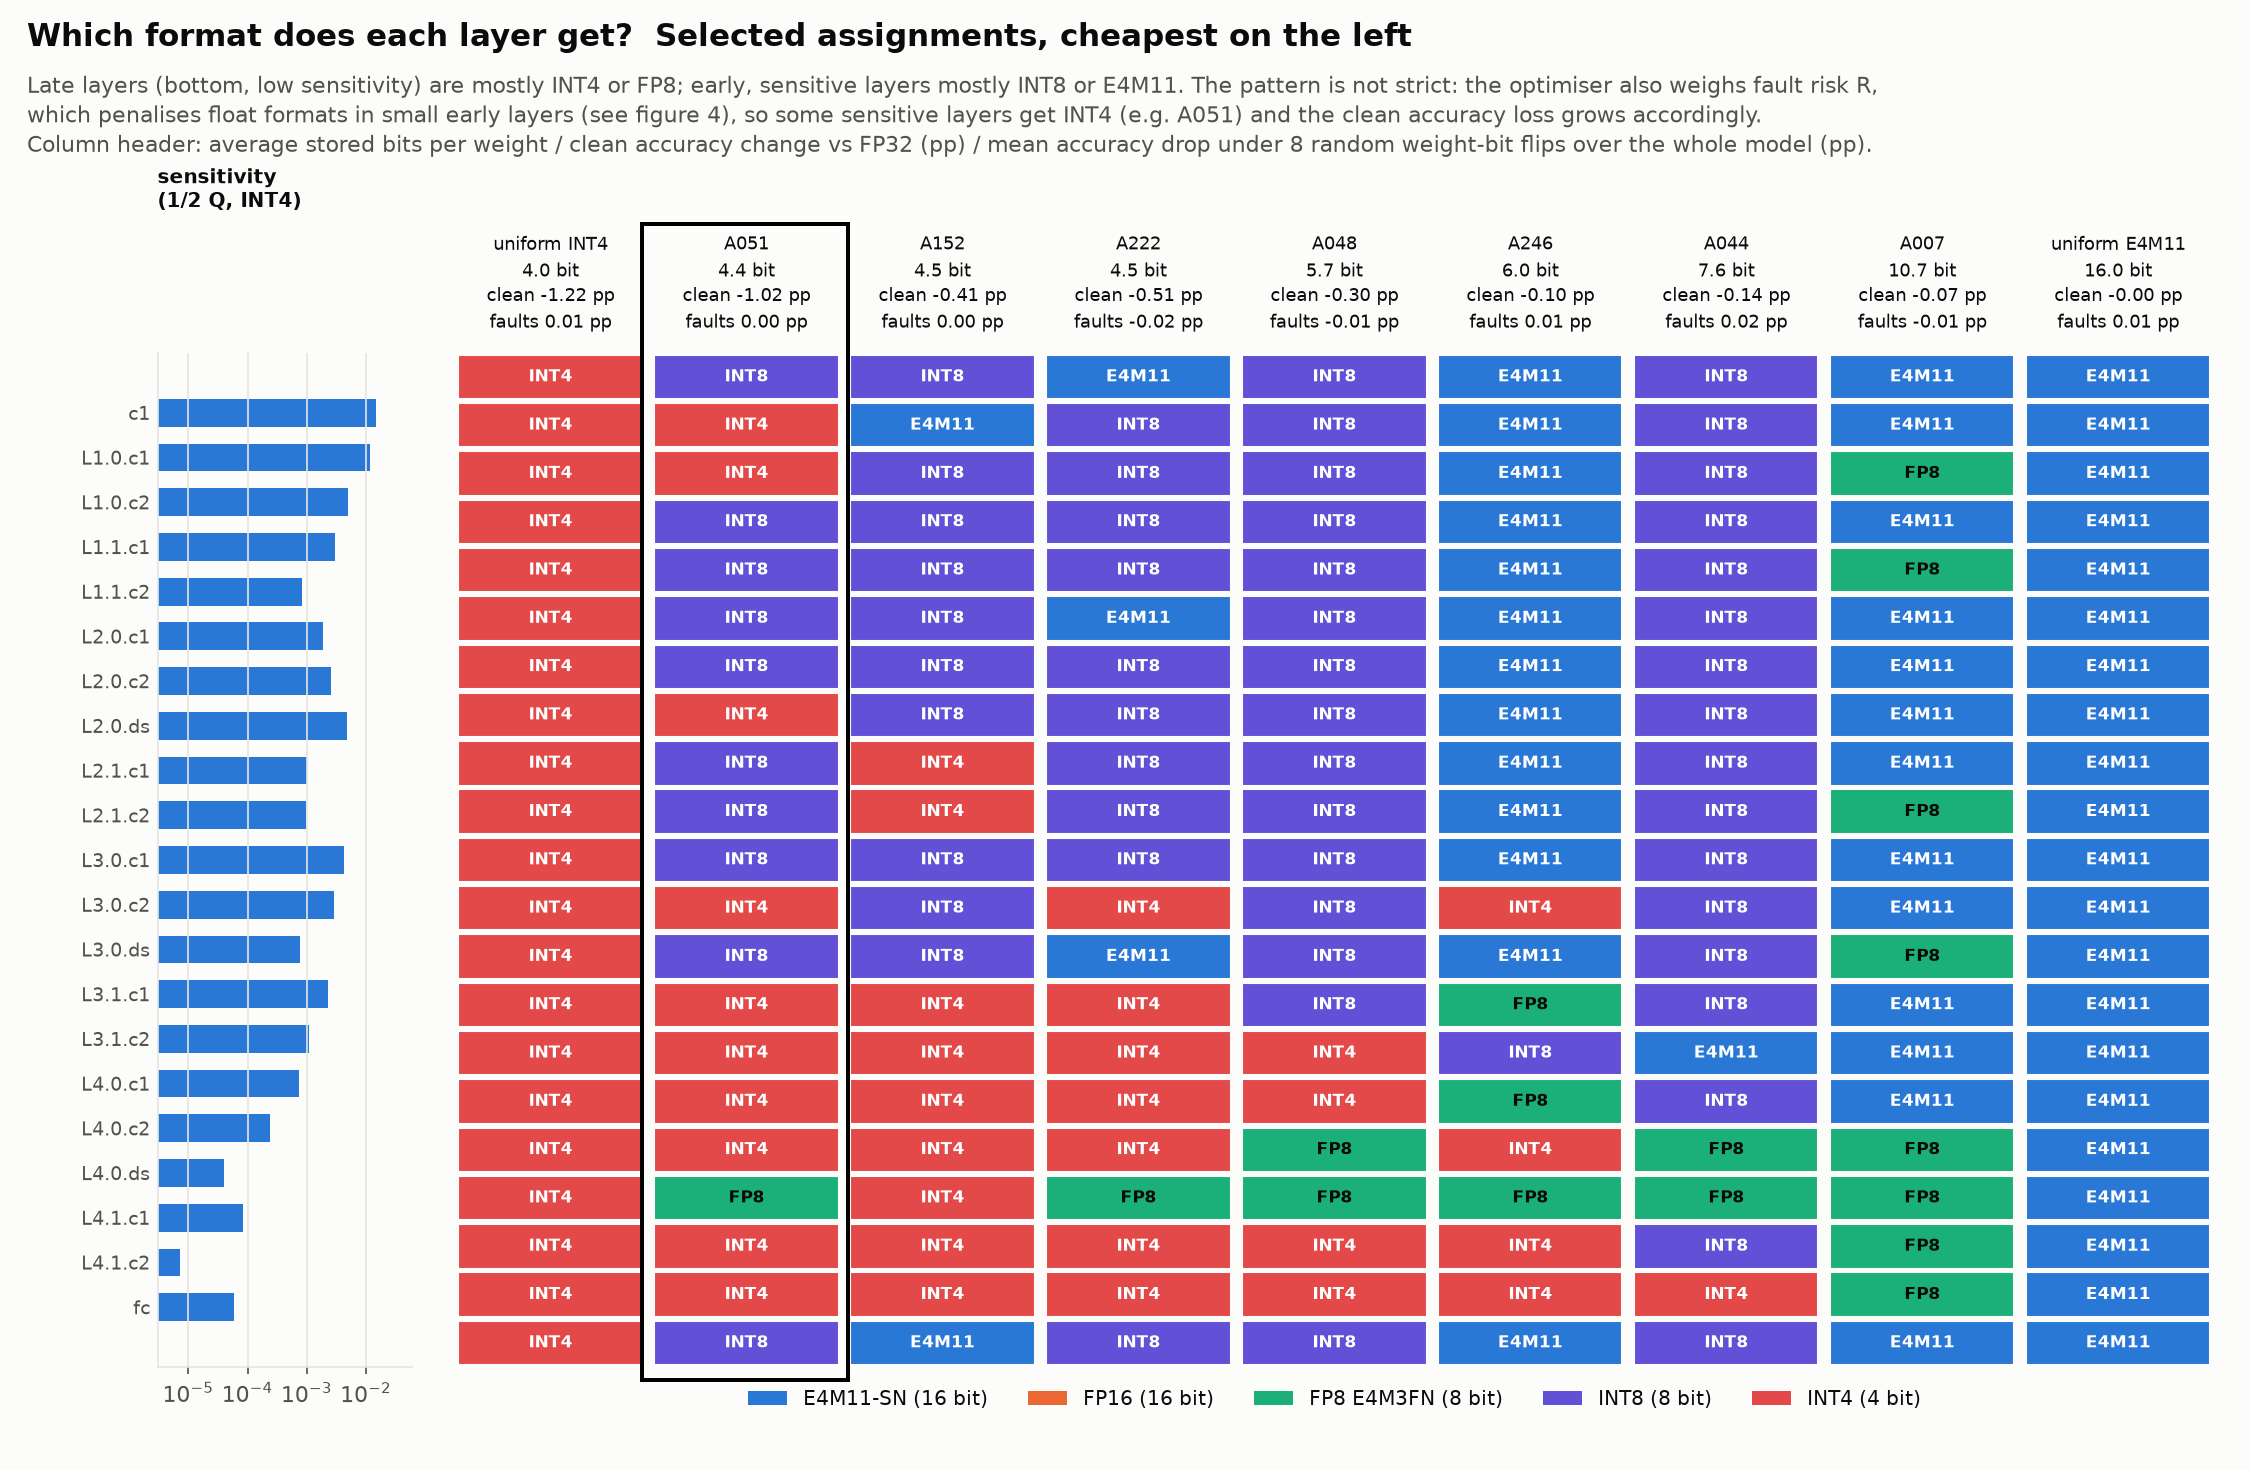
\includegraphics[width=0.78\textwidth,height=0.8\textheight,keepaspectratio]{rn_assignments_A051.png}\\[-1mm]
  {\scriptsize A051 (framed): 10 layers INT8, 10 layers INT4, 1 layer FP8 E4M3FN. Most early layers stay INT8 (exceptions: L1.0.c1, L1.0.c2, L2.0.ds are INT4); the large late layers become INT4, with L4.0.ds in FP8 and fc in INT8.
  Left: Fisher sensitivity of each layer for INT4 ($\tfrac12 Q$).}
\end{frame}

% ------------------------------------------------------------------ 8. A051 metrics
\begin{frame}{A051 compared with the FP32 model}
  \small
  Clean accuracy and SQNR on the 2\,952 validation images not used for the Fisher (images 2048--4999); faults on a 1\,000-image subset.\\[2mm]
  \begin{tabular}{@{}lrrr@{}}
    \toprule
    & FP32 baseline & A051 & change\\
    \midrule
    validation accuracy & 95.29\,\% & 94.28\,\% & $-1.02$ pp\\
    cross-entropy loss & 0.1760 & 0.1810 & $+0.0050$\\
    global SQNR & $+\infty$ dB & 9.38 dB & --\\
    weight storage & 44\,657\,408 B & 6\,109\,968 B & $7.3\times$ smaller ($-86.3\,\%$)\\
    average bits per weight & 32 & 4.38 & --\\
    8 random weight-bit flips, mean drop & -- & 0.002 pp & worst of 50 trials: 0.10 pp\\
    \bottomrule
  \end{tabular}\\[3mm]
  \begin{itemize}\small
    \item A051 is about as small as uniform INT4 (4.00 bit) but loses 1.02 pp instead of 1.22 pp, with a higher SQNR than uniform INT4 (9.38 vs 7.85 dB): it keeps INT8 in most early layers.
    \item Its SQNR is far below uniform INT8 (32.58 dB), yet the accuracy loss is only 1 pp: SQNR is not a good accuracy predictor.
    \item 8 random bit flips in the stored weights do not change its accuracy measurably (50 trials).
    \item \textbf{Caveat}: its INT layers keep an unprotected float32 scale; one flipped scale bit costs 8.7 pp on average (worst 71.7 pp, 50 trials).
    \item Test-set accuracy was not measured for A051 (the test set is read once, for the frozen final assignment).
  \end{itemize}
  {\footnotesize A051 comes from the first, datatype-only optimisation round (risk $R$ = mean single-layer 8-flip drop); a later round with protected scales supersedes it for the final assignment.}
\end{frame}

\end{document}
